\documentclass{article}
\title{Homework2.5}
\author{Blue}
\date{20230118}
\usepackage{geometry}
\geometry{a4paper,scale=0.8}
\usepackage{graphicx}
\usepackage{float}
\usepackage{indentfirst}
\usepackage[namelimits]{amsmath} %数学公式
\usepackage{amssymb}             %数学公式
\usepackage{color}
\usepackage{longtable}
\usepackage{listings}
\lstset{
language=Matlab,
numbers=left,
keywordstyle=\color{blue},
numberstyle=\tiny,
breaklines=true,
extendedchars=flase
}
\begin{document}
\maketitle
\section{Solve a differential equations.}
\begin{figure}[H]
\centering
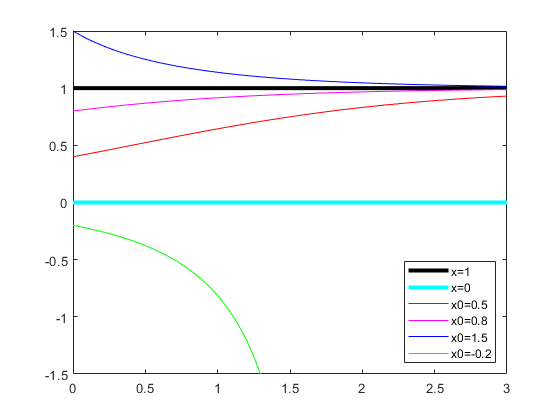
\includegraphics{results.png}
\caption{result}
\end{figure}
I choose 4 initial value, and get the results above. They behave the same as problem 3.a.1.
\section{code}
\begin{lstlisting}
t0=linspace(0,6,601);
x2=0*t0;
x1=0*t0+1;
plot(t0,x1,'Color','k','DisplayName','x=1','linewidth',3)
hold on
plot(t0,x2,'Color','c','DisplayName','x=0','linewidth',3)
ploty(0.4,0.01,3,'r','x0=0.5')
ploty(0.8,0.01,3,'m','x0=0.8')
ploty(1.5,0.01,3,'b','x0=1.5')
ploty(-0.2,0.01,1.3,'g','x0=-0.2')
axis([0,3,-1.5,1.5])
legend('Location','southeast')
hold off

function ploty(x0,h,ends,linecolor,xname)
tv=linspace(0,ends,ends/h+1);
xv=linspace(0,ends,ends/h+1);
tv(1)=0;
xv(1)=x0;
for i=2:ends/h+1
    tv(i)=h*(i-1);
    xv(i)=xv(i-1)+h*cal(xv(i-1));
end
plot(tv,xv,'Color',linecolor,'DisplayName',xname)
end

function xpr=cal(x)
xpr=x*(1-x);
end
\end{lstlisting}








\end{document}